% Options for packages loaded elsewhere
\PassOptionsToPackage{unicode}{hyperref}
\PassOptionsToPackage{hyphens}{url}
%
\documentclass[
]{article}
\usepackage{amsmath,amssymb}
\usepackage{lmodern}
\usepackage{iftex}
\ifPDFTeX
  \usepackage[T1]{fontenc}
  \usepackage[utf8]{inputenc}
  \usepackage{textcomp} % provide euro and other symbols
\else % if luatex or xetex
  \usepackage{unicode-math}
  \defaultfontfeatures{Scale=MatchLowercase}
  \defaultfontfeatures[\rmfamily]{Ligatures=TeX,Scale=1}
\fi
% Use upquote if available, for straight quotes in verbatim environments
\IfFileExists{upquote.sty}{\usepackage{upquote}}{}
\IfFileExists{microtype.sty}{% use microtype if available
  \usepackage[]{microtype}
  \UseMicrotypeSet[protrusion]{basicmath} % disable protrusion for tt fonts
}{}
\makeatletter
\@ifundefined{KOMAClassName}{% if non-KOMA class
  \IfFileExists{parskip.sty}{%
    \usepackage{parskip}
  }{% else
    \setlength{\parindent}{0pt}
    \setlength{\parskip}{6pt plus 2pt minus 1pt}}
}{% if KOMA class
  \KOMAoptions{parskip=half}}
\makeatother
\usepackage{xcolor}
\IfFileExists{xurl.sty}{\usepackage{xurl}}{} % add URL line breaks if available
\IfFileExists{bookmark.sty}{\usepackage{bookmark}}{\usepackage{hyperref}}
\hypersetup{
  pdftitle={Hypothesis Tests With Separation},
  pdfauthor={Carlisle Rainey},
  hidelinks,
  pdfcreator={LaTeX via pandoc}}
\urlstyle{same} % disable monospaced font for URLs
\usepackage[margin=1in]{geometry}
\usepackage{graphicx}
\makeatletter
\def\maxwidth{\ifdim\Gin@nat@width>\linewidth\linewidth\else\Gin@nat@width\fi}
\def\maxheight{\ifdim\Gin@nat@height>\textheight\textheight\else\Gin@nat@height\fi}
\makeatother
% Scale images if necessary, so that they will not overflow the page
% margins by default, and it is still possible to overwrite the defaults
% using explicit options in \includegraphics[width, height, ...]{}
\setkeys{Gin}{width=\maxwidth,height=\maxheight,keepaspectratio}
% Set default figure placement to htbp
\makeatletter
\def\fps@figure{htbp}
\makeatother
\setlength{\emergencystretch}{3em} % prevent overfull lines
\providecommand{\tightlist}{%
  \setlength{\itemsep}{0pt}\setlength{\parskip}{0pt}}
\setcounter{secnumdepth}{-\maxdimen} % remove section numbering
\ifLuaTeX
  \usepackage{selnolig}  % disable illegal ligatures
\fi

\title{Hypothesis Tests With Separation}
\author{Carlisle Rainey\footnote{Carlisle Rainey is Associate Professor
  of Political Science, Florida State University, 540 Bellamy,
  Tallahassee, FL, 32306.
  (\href{mailto:crainey@fsu.edu}{crainey@fsu.edu}).}}
\date{}

\begin{document}
\maketitle

\begin{center}\rule{0.5\linewidth}{0.5pt}\end{center}

\begin{quote}
Draft under development. It's no doubt filled with typos and errors. This is the version from \today.
\end{quote}

\begin{center}\rule{0.5\linewidth}{0.5pt}\end{center}

\begin{center}
Word Count: input{doc/misc/word-count}
\end{center}

Separation commonly occurs in political science, usually when the
presence (or absence) of a binary explanatory variable perfectly
predicts the presence or absence of a binary outcome {[}e.g.,
@BellMiller2015; @Mares2015; @ViningWilhelmCollens2015{]}. For example,
@BarrilleauxRainey2014 find that being a Democrat perfectly predicts a
governor accepting Medicaid funds under the Affordable Care Act. Under
separation, the usual maximum likelihood estimates are unreasonably
large and the Wald \(p\)-values are highly misleading.

As a solution, some methodologists propose using a Bayesian prior
distribution to regularize the estimates, which we can alternatively
consider as \emph{penalized} maximum likelihood estimator. @Zorn2005
{[}see also @HeinzeSchemper2002{]} points political scientists toward
the penalized maximum likelihood estimator proposed by @Firth1993, which
is equivalent to Jeffreys' prior distribution {[}@Jeffreys1946{]}. As an
alternative, @Gelmanetal2008 recommend a Cauchy prior distribution. Both
of these methods ensure finite estimates in theory and usually produce
reasonably-sized estimates in practice.

But @Rainey2016 points out that the parameter estimates (and especially
the confidence intervals) depend largely on the chosen prior
distribution or penalty. Indeed, many priors that guarantee finite
estimates can lead to meaningfully different conclusions. He argues that
the set of \emph{a priori} ``reasonable'' and ``implausible'' parameters
depends on the substantive application, so context-free defaults (like
Jeffreys' and Cauchy priors) might not produce reasonable results.
@Rainey2016 concludes that ``{[}w{]}hen facing separation, researchers
must \emph{carefully} choose a prior distribution to nearly rule out
implausibly large effects'' (p.~354).

But it's not always easy to include prior information, and some scholars
prefer to avoid injecting prior information into their model. How can
researchers proceed in these situations? In particular, can they obtain
useful \(p\)-values to test hypotheses in the usual frequentist
framework without using prior information?

Below, I show that while the popular Wald test produces misleading (even
nonsensical) \(p\)-values under separation, likelihood ratio tests and
score tests behave in the usual manner. As such, researchers can produce
meaningful \(p\)-values to test hypotheses with standard frequentist
tools under separation \emph{without the use of prior information}.

\hypertarget{statistial-theory}{%
\section{Statistial Theory}\label{statistial-theory}}

\hypertarget{point-estimates}{%
\subsection{Point Estimates}\label{point-estimates}}

Maximum likelihood provides a general and powerful framework for
obtaining estimates of model parameters. In our case of logistic
regression, we write the probability \(\pi_i\) that an event occurs for
observation \(i\) (or that the outcome variable \(y_i = 1\)) as

\begin{equation}
\pi_i = \text{logit}^{-1}(X_i\beta)\text{ for } i = 1, 2, ... , n \text{, }
\end{equation}

\noindent where \(X\) represents a matrix of explanatory variables and
\(\beta\) represents a vector of coefficients. Then we can derive the
likelihood function \(L(\beta | y)\)

\begin{equation}
L(\beta | y) = \pi_{i}^{y_i}(1 - \pi_{i})^{(1 - y_i)}\text{,  where } \pi_i = \text{logit}^{-1}(X_i\beta)
\end{equation}

\noindent and the log-likelihood function

\begin{equation}
\ell(\beta | y) = \log L(\beta | y) = y_i \log(\pi_{i}) + (1 - y_i) \log(1 - \pi_{i}).
\end{equation}

For logistic regression (and many other models), researchers typically
use numerical algorithms to locate the value \(\hat{\beta}^{ML}\) of
\(\beta\) that maximizes \(\ell\). For examples, Stata's \texttt{logit}
command used a modified Newton-Raphson algorithm
(\href{https://www.stata.com/help.cgi?maximize\#GPP2010}{link}) and R's
\texttt{glm()} function uses iteratively reweighted least squares. Then,
to test hypotheses, we rely on certain features of \(\ell\), depending
on the test.

\hypertarget{hypothesis-tests}{%
\subsection{Hypothesis Tests}\label{hypothesis-tests}}

With the point estimates in hand, researchers typically compare their
research hypothesis \(H_R\) to a null hypothesis \(H_0\). For a logistic
regression, the researcher might compose a null hypothesis as
\(H_0: \beta \in B_0 \subset R^n\), which leaves the research hypothesis
as \(H_R: \beta \in B_0^C\). Depending on the data, the researcher may
then choose to reject \(H_0\) in favor of \(H_R\) or fail to distinguish
between the two.

To fix ideas, I focus on the simple point null hypothesis
\(H_0: \beta_s = 0\). However, the intuition and conclusions generalize
to more complex hypotheses.

The literature offers three common methods to assess the null
hypothesis---the ``holy trinity'' of hypothesis tests: the Wald test,
the likelihood ratio test, and the score test. For practical reasons,
most regression tables in political science include \(p\)-values and
stars based on the Wald test. While usually the most convenient of the
three tests, the Wald test is uniquely ill-suited for testing hypotheses
under separation. The likelihood ratio and score tests, on the other
hand, work as expected. Below I briefly describe each test, explain why
the Wald test works poorly under separation, and describe why the
likelihood ratio and score tests perform better.

\hypertarget{wald-test}{%
\subsubsection{Wald Test}\label{wald-test}}

Of the three methods, researchers usually report the Wald test because
it requires fitting only the full model. The Wald procedure uses the
shape of the log-likelihood function around the maximum to estimate the
precision of the point estimate. If small changes in the parameter near
the maximum lead to large changes in the log-likelihood function, then
we can treat the maximum likelihood estimate as precise. However, if
large changes in the parameter lead to small changes in the likelihood
function, then we must treat the maximum likelihood estimate as
imprecise.

More formally, the Wald test uses the second derivative to quantify the
curvature of \(\ell\) at \(\hat{\beta}^{ML}\). Further, we can estimate
the standard error \(\widehat{\text{SE}}(\hat{\beta}_i^{ML})\) as

\begin{equation}\label{eqn:ml-se}
\widehat{\text{SE}} \left( \hat{\beta}_i^{ML} \right) = \left( - \dfrac{\partial^2 \ell(\hat{\beta}_i^{ML} | y)}{\partial^2 \hat{\beta}_i^{ML}} \right)^{-\frac{1}{2}}\text{.}
\end{equation}

For large samples, the maximum likelihood estimate approximately follows
a normal distribution centered at the true value of \(\beta\) with a
standard deviation of \(\widehat{\text{SE}}(\hat{\beta}_i^{ML})\). Wald
(1943) advises us how compare the estimate with the standard error: the
statistic
\(Z_w = \dfrac{\hat{\beta}_i^{ML}}{\widehat{\text{SE}}(\hat{\beta}_i^{ML})}\)
follows a standard normal distribution approximate follows a standard
normal distribution. (Casella and Berger 2003, pp.~???, Greene 2012,
pp.~527-529).

However, \emph{this approach works poorly when dealing with separation}.
Under separation, the log-likelihood function at the found maximum is
numerically flat or nearly so. The flatness produces very large standard
error estimates, which has a troubling dependence on the error tolerance
of the algorithm.

For a logistic regression model with a separating variable, we can state
a precise result that relates the size of the coefficient of the
separating variable to the Wald estimate of its standard error.

\begin{theorem}\label{thm:growth}
Suppose that a binary explanatory variable $s$ with coefficient $\beta_s$ perfectly predicts the outcome $y_i$ such that when $s_i = 1$ then $y_i = 1$. Then the log-likelihood function increases in $\beta_s$ and the quantity $\lim_{\beta_s \to \infty} \left[ \left( - \dfrac{\partial^2 \ell(\beta_s | y)}{\partial^2 \beta_s} \right)^{-\frac{1}{2}} - \beta_s \right] = \infty$. Thus, under separation, the estimated standard error will be much larger than the coefficient for the separating variable for any algorithm that obtains a sufficiently large coefficient.
\end{theorem}

\noindent Theorem \ref{thm:growth} shows that, so long as the researcher
uses a sufficiently precise algorithm, the Wald test will \emph{never}
reject the null hypothesis.

Theorem \ref{thm:growth} has an important practical implication, given
in Corrollary \ref{cor:bound}.

\begin{corrollary}\label{cor:bound}
Suppose a data-generating process that results in separation with probability $p$. Then the power of the Wald test cannot exceed $1 - p$.
\end{corrollary}

This has a counter-intuitive implication that highlights the poor
behavior of the Wald test under separation. Increasing the coefficient
of a potentially separating variable increases the chance of separation.
But Corrollary \ref{cor:bound} established that this must
\emph{decrease} the power of the test. This leads to a pathological
result, moving the coefficient further from zero must \emph{decrease}
the power of the test.

Figure \ref{fig:trinity} shows this intuition for a typical,
non-monotonic log-likelihood function (i.e., without separation) and for
a monotonic log-likelihood function (i.e., with separation). In the
absence of separation, the curvature of the log-likelihood function
around the maximum speaks to the evidence against the null hypothesis.
But under separation, the likelihood function, \emph{by definition}, is
flat at the maximum, regardless of the relative likelihood of the data
under the null hypothesis.

\begin{figure}[h]
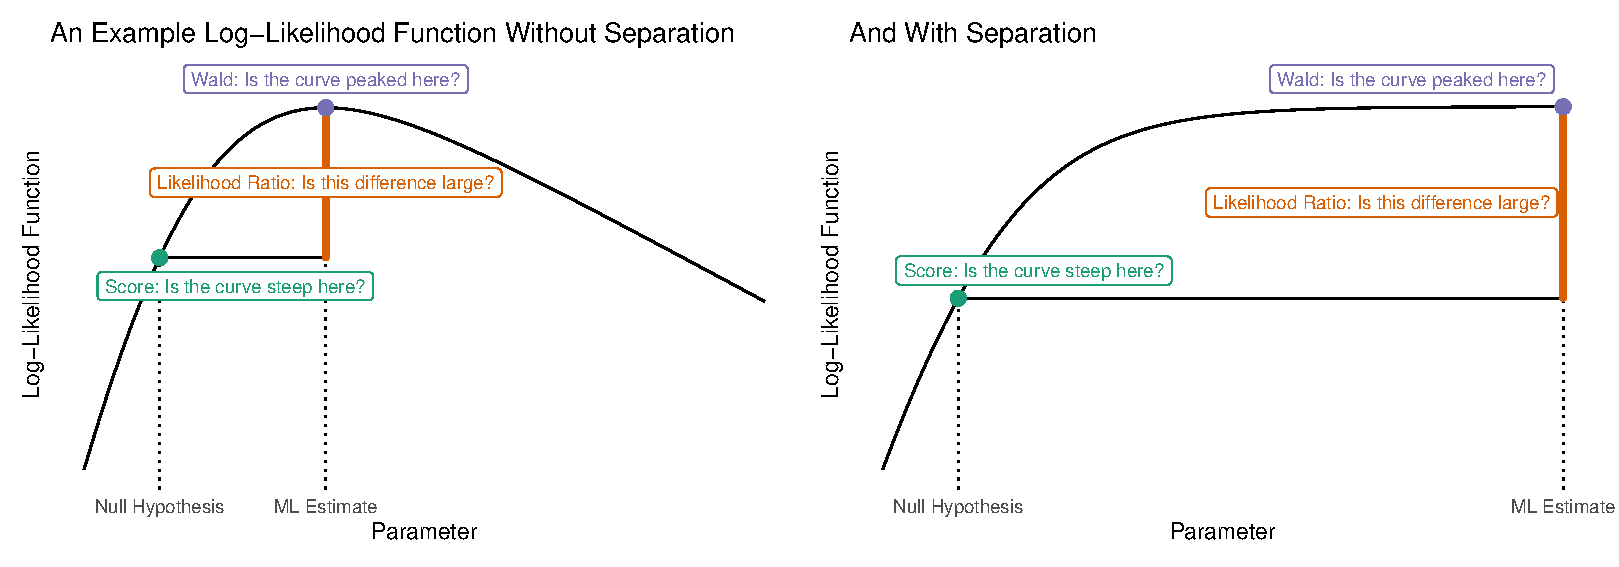
\includegraphics[width=\textwidth]{doc/fig/intuition.pdf}
\caption{A figure summarizing logic of the "holy trinity" of hypothesis tests. The Wald test relies on the curvature around the maximum of the log-likelihood function, which breaks down under separation. But the likelihood ratio and score test rely on \textit{other} features of the log-likelihood function, that are not meaningfully impacted by separation.}\label{fig:trinity}
\end{figure}

To see the importance of this result, suppose an absurd example in which
a binary treatment perfectly predicts 500 successes and 500 failures
(i.e., \(y = x\) always). Of course, these data are \emph{extremely}
unlikely under the null hypothesis that the coefficient for the
treatment indicator equals zero. The exact \(p\)-value for the null
hypothesis that successes and failures are equally likely under both
treatment and control equals
\(2 \times \left( \frac{1}{2} \right)^{500} \times \left( \frac{1}{2} \right)^{500} = \frac{2}{2^{1000}} \approx \frac{2}{10^{301}}\).
(For comparison, there are about \(10^{80}\) atoms in the known
universe.) Yet, the default \texttt{glm()} routine in R calculates a
Wald \(p\)-value of 0.998 with the default precision and 1.000 with the
maximum precision.

When dealing with separation, the approach of using curvature around the
maximum to estimate the relative likelihood of the restricted model
breaks down; researchers cannot use the Wald test to obtain reasonable
\(p\)-values for the coefficient of a separating variable.

\hypertarget{likelihood-ratio-test}{%
\subsubsection{Likelihood Ratio Test}\label{likelihood-ratio-test}}

The likelihood ratio test resolves the problem of the flat
log-likelihood by comparing the maximum log-likelihood of two models: an
``unrestricted'' model \(ML\) that imposes no bounds on the estimates
and a ``restricted'' model \(ML_0\) that constrains the estimates to the
region suggested by the null hypothesis. If the data are much more
likely under the unrestricted estimate than under the restricted
estimate, then the researcher can reject the null hypothesis.

More formally, the likelihood ratio test compares the value of the
unrestricted log-likelihood \(\ell(\hat{\beta}^{ML} | y)\) to the
restricted log-likelihood \(\ell(\hat{\beta}^{ML_0} | y)\). For the
simple null hypothesis \(H_0: \beta_s = 0\), we can understand \(ML_0\)
as a separate model fit without the explanatory variable \(s\).

Wilks' theorem (1938) advises us how to compare the two likelihoods:
\(D = 2 \times \left[ \ell(\hat{\beta}^{ML} | y) - \ell(\hat{\beta}^{ML_0} | y) \right]\)
follows a \(\chi^2\) distribution with degrees of freedom equal to the
number of constrained dimensions (Casella and Berger 2003, pp.~488-492,
Greene 2003, pp.~484-486).

Figure \ref{fig:trinity} also shows the intuition of the likelihood
ratio test. The figure highlights that the gap between the unrestricted
and restricted maximum summarizes the evidence against the null
hypothesis. Further, the logic does not break down under separation.
Unlike the Wald test, the likelihood ratio test can reject the null
hypothesis under separation.

\hypertarget{score-test}{%
\subsubsection{Score Test}\label{score-test}}

The score test resolves the problem of the flat log-likelihood by
focusing on gradient of the log-likelihood function at the null
hypothesis. If the null hypothesis is correct, then the log-likelihood
should not be increasing much around that point. But if the
log-likelihood function is increasing rapidly at the null hypothesis,
this casts doubt on the null hypothesis. The score test uses two
quantities: the score function
\(S(\beta) = \dfrac{\partial \ell(\beta | y)}{\partial \beta}\) and the
Fisher information
\(I(\beta) = -E_\beta \left( \dfrac{\partial^2 \ell(\beta | y)}{\partial^2 \beta} \right)\).
When evaluated at the null hypothesis, the score function quantifies the
slope and the Fisher information quantifies the variance of that slope
in repeated samples.

If the score at the null hypothesis is large relative to its standard
deviation, then researchers can reject the null hypothesis. Rao (1948)
advises us how evaluate the assess the statistic:
\(Z_s = \frac{S(\beta^0_s)}{\sqrt{I(\beta^0_s)}}\) follows a standard
normal distribution. (Rao 1948, Casella and Berger 2003, pp.~494-495,
Greene 2003, pp.~489-490).

Figure \ref{fig:trinity} finally shows the intuition of the score test.
The figure highlights that the slope of the log-likelihood function
under the null hypothesis summarizes the evidence against the null
hypothesis. As with the likelihood ratio test, the logic works even
under separation, and the score test can reject the null hypothesis
under separation.

Table \ref{tab:trinity} summarizes the three tests. Most importantly,
the likelihood ratio and score test rely on features of the
log-likelihood function that are not meaningfully affected by a
monotonic log-likelihood function created by separation. The Wald test,
on the other hand, cannot provide a reasonable tests under separation
(see Theorem \ref{thm:growth}). For more details on the three tests, see
Silvey (1959) or Greene (2012, pp.~524--530).

\begin{table}[h]
\footnotesize
\begin{tabular}{{p{0.1\textwidth}p{0.3\textwidth}p{0.5\textwidth}}}
Test & Feature                                                      & Statistic and Distribution      \\
\hline                                                                                  
Wald & Curvature of the log-likelihood function around the maximum. & $Z_w = \dfrac{\hat{\beta}_i^{ML}}{\widehat{\text{SE}}(\hat{\beta}_i^{ML})}$ follows a standard normal distribution.\\
 Likelihood Ratio    &   Relative log-likelihoods of the unrestricted and restricted models. &  $D = 2 \times \left[ \ell(\hat{\beta}^{ML} | y) - \ell(\hat{\beta}^{ML_0} | y) \right]$ follows a $\chi^2$ distribution with degrees of freedom equal to the number of constrained dimensions. \\
 Score    &   Slope of the log-likelihood function \textit{at the null hypothesis}.                                                            &   $Z_s = \frac{S(\beta^0_s)}{\sqrt{I(\beta^0_s)}}$ follows a standard normal distribution.
\end{tabular}\caption{A table summarizing the "holy trinity" of hypothesis tests.}\label{tab:trinity}
\end{table}

\hypertarget{simulations}{%
\section{Simulations}\label{simulations}}

To evaluate the performance of the various methods for testing
hypothesis under separation, I use a diverse collection of
data-generating processes (DGPs) that feature separation in more than
10\% of repeated samples. Importantly, I cannot focus on data sets
\emph{with separation} because separation is a feature of a particular
sample. Instead, I focus on DGPs that \emph{sometimes} feature
separation (e.g., in 15\% of repeated samples, in 50\% of repeated
samples, etc.).

To create the collection of DGPs, I imagine the logistic regression
model
\(\Pr(y = 1) = \text{logit}^{-1}(\beta_{\text{cons}} + \beta_s s + \beta_{z_1} z_1 + ... + \beta_{z_k} z_k)\)
and a researcher testing the null hypothesis that the binary explanatory
variable \(s\) (that might produce separation) has no effect on a binary
outcome variable \(y\). I vary the frequency that \(s = 1\), the value
of \(\beta_{\text{cons}}\), the number of control variables (\(k\)), and
the total number of observations. For each DGP, I use Monte Carlo
simulation to compute the power function as \(\beta_s\) varies for each
of the three tests: Wald test, likelihood ratio test, and score test.
For completeness, I also compute the power function for Wald tests using
the two Firth and Cauchy PML estimates.

I use all 944 (logically possible) combinations of the values below.
When the null hypothesis true (i.e., \(\beta_s = 0\)), the percent of
repeated samples with separation ranges from 98\% (ctk) to 14\% (ctk) in
this collection.

\hypertarget{a-close-look-at-a-single-dgp}{%
\subsection{A Close Look at a Single
DGP}\label{a-close-look-at-a-single-dgp}}

To clarify the simulation results, I provide the details for a single
DGP. Following the structure discussed above, Table
\ref{tab:single-dgp-pars} shows the parameters for this single DGP.

\renewcommand{\captiontext}{}
\renewcommand{\notetext}{}
\begin{table}[!h]
\caption{\label{tab:single-dgp-pars}}
\centering
\fontsize{10}{12}\selectfont
\begin{threeparttable}
\begin{tabular}{lc}
\toprule
Parameter & Value        \\
\midrule
Total Number of Observations & 50 \\
Frequency that $s = 1$    &   5 \\
The Value of the Intercept $\beta_{\text{cons}}$ & 0 \\
The Number of Control Variables $k$ & 2 \\
\bottomrule
\end{tabular}\begin{tablenotes}[para]

\end{tablenotes}
\end{threeparttable}
\end{table}

Table \ref{tab:single-dgp-pwr} shows the power function for each of the
three tests, as well as the ideal power, and the percent of the data
sets that featured separation for the parameter combination and the
value of \(\beta_s\). For this particular DGP, separation is relatively
rare when \(\beta_s\)---the coefficient for the potentially separating
variable---is near zero. But for \(\beta_s = \pm 2\), about 50\% of the
data sets feature separation. And for \(\beta_s\) larger/smaller than
\(\pm 4\), more than 90\% of the data sets feature separation.

This DGP clearly shows the implication if Theorem \ref{thm:growth}. Even
though the data sets with separation should allow the researcher to
reject the null hypothesis, at occasionally, the power of the Wald test
is near 0\%, even for very large effects. The likelihood ratio and score
tests, on the other hand, perform as expected. For both alternatives,
the power of the test when \(\beta_s = 1\) is about 5\%, as designed,
and the power approaches 100\% relatively quickly as \(\beta_s\) moves
away from zero. For this particular DGP, the likelihood ratio is a more
powerful test, than the score test, but the likelihood ratio and score
tests work reasonably well, unlike the Wald test.

\renewcommand{\captiontext}{}
\renewcommand{\notetext}{This table shows the power for the Wald, likelihood ratio, and score tests for a DGP that often features separation.}
\begin{table}[!h]
\caption{\label{tab:single-dgp-pwr}}
\centering
\fontsize{10}{12}\selectfont
\begin{threeparttable}

\begin{tabular}{>{}cccccccc}
\toprule
$\beta_s$ & Ideal Power & Chance of Separation & ML w/ Wald & ML w/ LR & ML w/ Score & PML (Firth) w/ Wald & PML (Cauchy) w/ Wald\\
\midrule
5.00 &  & 81\% & 20\% & 100\% & 100\% & 100\% & 100\%\\

4.00 &  & 58\% & 43\% & 100\% & 100\% & 99\% & 99\%\\

3.00 &  & 25\% & 72\% & 98\% & 98\% & 95\% & 96\%\\

2.00 &  & 3\% & 71\% & 76\% & 77\% & 68\% & 70\%\\

1.00 &  & 0\% & 26\% & 28\% & 30\% & 22\% & 22\%\\

0.75 &  & 0\% & 16\% & 17\% & 19\% & 13\% & 14\%\\

0.50 &  & 1\% & 10\% & 11\% & 12\% & 8\% & 8\%\\

0.40 &  & 1\% & 7\% & 9\% & 9\% & 5\% & 5\%\\

0.30 &  & 1\% & 6\% & 8\% & 8\% & 5\% & 5\%\\

0.20 &  & 2\% & 5\% & 7\% & 6\% & 4\% & 4\%\\

0.10 & \multirow{-11}{*}{\centering\arraybackslash As high as possible.} & 2\% & 3\% & 7\% & 6\% & 3\% & 3\%\\
\addlinespace
0.00 & 5\% & 3\% & 2\% & 6\% & 5\% & 2\% & 2\%\\
\addlinespace
-0.10 &  & 4\% & 2\% & 6\% & 4\% & 2\% & 2\%\\

-0.20 &  & 5\% & 2\% & 10\% & 6\% & 2\% & 2\%\\

-0.30 &  & 6\% & 1\% & 9\% & 6\% & 1\% & 1\%\\

-0.40 &  & 8\% & 1\% & 9\% & 5\% & 1\% & 1\%\\

-0.50 &  & 10\% & 1\% & 12\% & 6\% & 1\% & 1\%\\

-0.75 &  & 16\% & 1\% & 18\% & 10\% & 1\% & 2\%\\

-1.00 &  & 23\% & 0\% & 25\% & 15\% & 0\% & 2\%\\

-2.00 &  & 56\% & 0\% & 54\% & 30\% & 1\% & 5\%\\

-3.00 &  & 80\% & 0\% & 76\% & 42\% & 1\% & 6\%\\

-4.00 &  & 92\% & 0\% & 86\% & 48\% & 1\% & 6\%\\

-5.00 & \multirow{-11}{*}{\centering\arraybackslash As high as possible.} & 97\% & 0\% & 90\% & 51\% & 1\% & 6\%\\
\bottomrule
\end{tabular}   
\begin{tablenotes}[para]
This table shows the power for the Wald, likelihood ratio, and score tests for a DGP that often features separation.
\end{tablenotes}
\end{threeparttable}
\end{table}

\hypertarget{a-broad-look-at-many-dgps}{%
\subsection{A Broad Look at Many DGPs}\label{a-broad-look-at-many-dgps}}

Table \ref{tab:tab:many-dgps-pars} shows the broad collection of
parameters I used in the simulations. All combinations of the values
below yield 150 unique combinations. I excluded combinations in which
the frequency that \(s = 1\) exceeded the number of observations, which
leaves 110 combinations. For each of these 110 combinations, I use Monte
Carlo simulations to estimate the probability that each method rejects
the null hypothesis as the coefficient \(\beta_s\) varies from -10 to 10
(across the particular values shown in Table \ref{tab:single-dgp-pwr}).
I also exclude any scenario in which the parameter and the coefficient
\(\beta_s\) would sometimes produce data sets with no variation in the
outcome variable. As such, one might consider this a diverse collection
of DGPs that sometimes generate separation but almost always have
variation in the outcome.

\renewcommand{\captiontext}{}
\renewcommand{\notetext}{}
\begin{table}[!h]
\caption{\label{tab:many-dgps-pars}}
\centering
\fontsize{10}{12}\selectfont
\begin{threeparttable}
\begin{tabular}{lc}
\toprule
Parameter & Value        \\
\midrule
Total Number of Observations & 50, 250, 500 \\
Frequency that $s = 1$    &   5, 25, 50, 100, 250 \\
The Value of the Intercept $\beta_{\text{cons}}$ & -8, -5, -2.5, -1, 0 \\
The Number of Control Variables $k$ & 2, 6 \\
\bottomrule
\end{tabular}\begin{tablenotes}[para]

\end{tablenotes}
\end{threeparttable}
\end{table}

Figure \ref{fig:many-sims} shows the statistical power of each of the
three tests as the chance of separation varies. Most starkly, the power
of the Wald test is bounded above my the chance of separation.
Intuitively, as the coefficient of the potential separating variable
increases, the power of the test should \emph{increase}. But because a
large coefficient makes separation more likely, a large coefficient
\emph{decreases} the power of the test. The likelihood ratio and score
test behave as expected.

\begin{figure}[h]
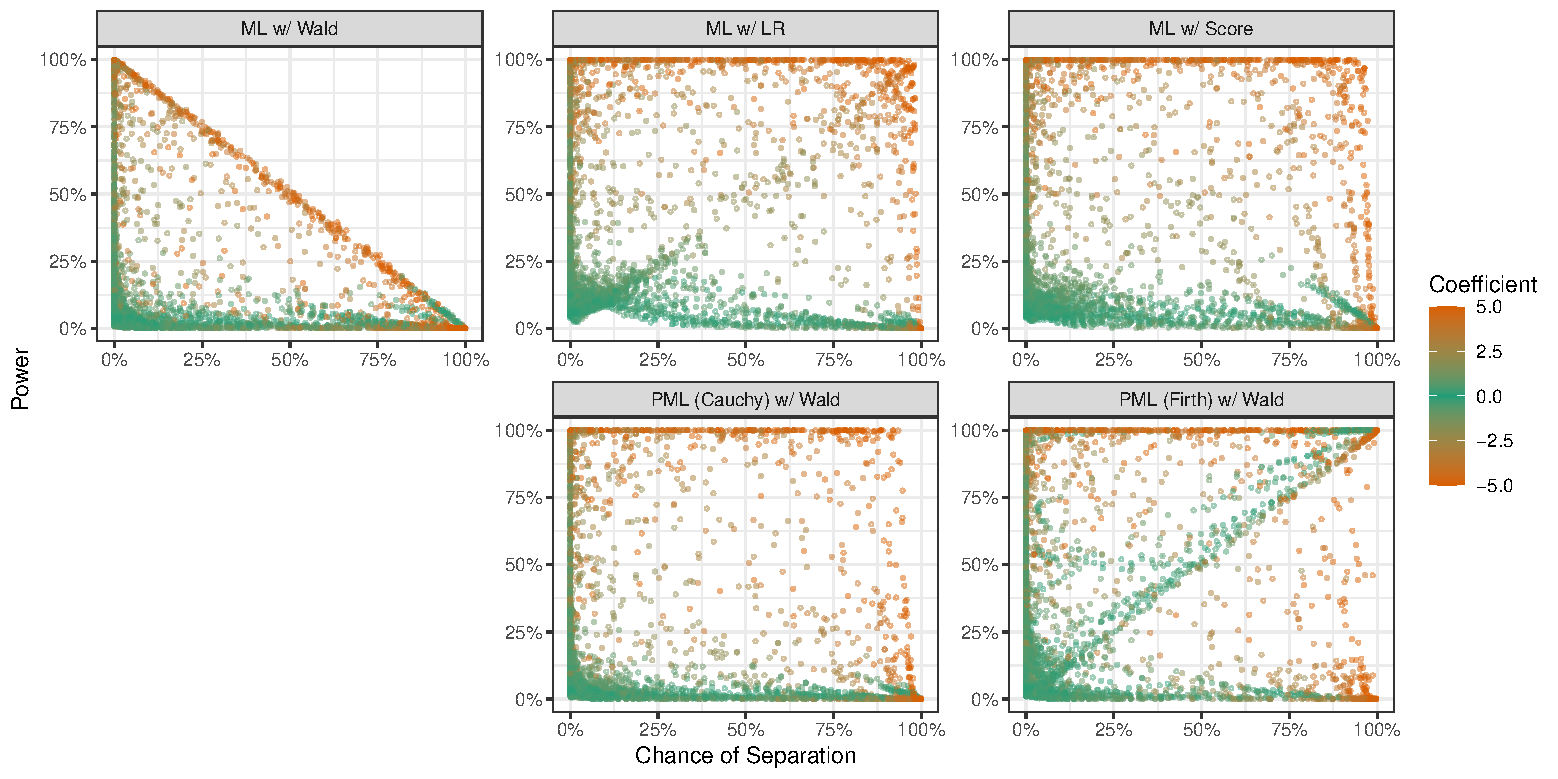
\includegraphics[width=\textwidth]{doc/fig/many-sims.pdf}
\caption{caption here}\label{fig:many-sims}
\end{figure}

Figure \ref{fig:power-funs}

\begin{figure}[h]
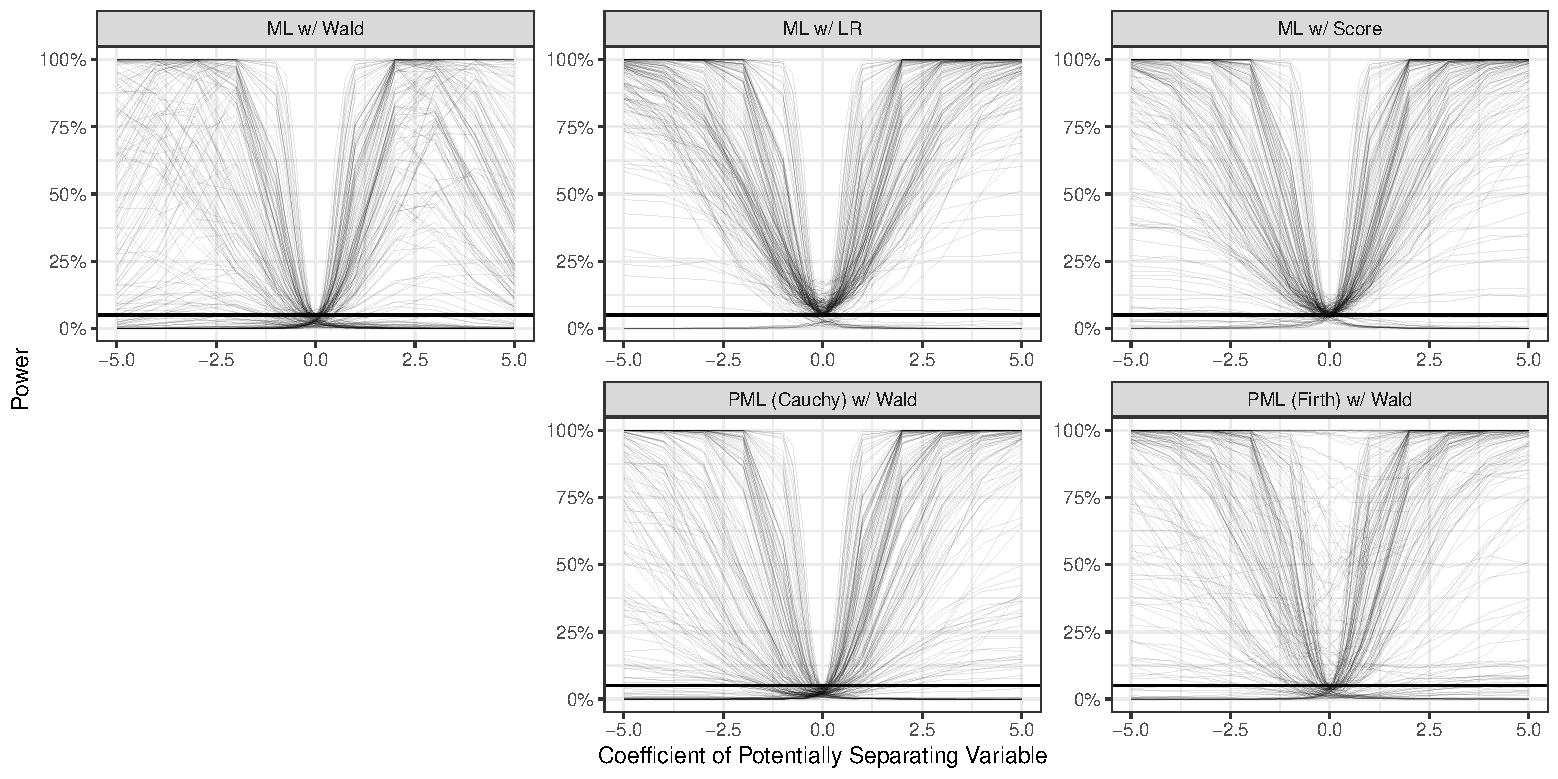
\includegraphics[width=\textwidth]{doc/fig/power-funs.pdf}
\caption{caption here}\label{fig:power-funs}
\end{figure}

\hypertarget{re-analysis-of-barrilleaux-and-rainey-2014}{%
\subsection{Re-Analysis of Barrilleaux and Rainey
(2014)}\label{re-analysis-of-barrilleaux-and-rainey-2014}}

To illustrate frequentist hypothesis testing under separation, I
reanalyze data from @BarrilleauxRainey2014 (that @Rainey2016 considers
in great detail). @BarrilleauxRainey2014 examine U.S. state governors
decisions to support or oppose the Medicaid expansion under the 2010
Affordable Care Act. But because all Democratic governors supported the
expansion, separation occurs---being a Democratic governor perfectly
predicts support for Medicaid expansion.

I focus on their first hypothesis: \emph{Republican governors are more
likely to oppose the Medicaid expansion funds than Democratic
governors.} Barrilleaux and Rainey adopt a fully Bayesian approach,
modeling the probability that a state's governor opposes the Medicaid
expansion as a function of the governor's partisanship and several other
covariates. Here, I re-estimate their logistic regression model using
several frequentist procedures. The appendix provides the full details.
Table \ref{tab:br-p} presents the estimates and \(p\)-values for the
coefficient of the binary Democratic governor variable.

\renewcommand{\captiontext}{}
\renewcommand{\notetext}{This table shows the $p$-values from several procedures that researchers might use when dealing with separation in logistic regression models. The Wald test for maximum likelihood estimates relies on unreasonable standard errors that depend heavily on the precision of the algorithm and, as a consequence, produces unrealistic $p$-values. However, the $p$-values from the likelihood ratio test seem reasonable and resemble the $p$-vales from the more conservative penalized maximum likelihood approaches.}
\begin{table}[!h]
\caption{\label{tab:br-p}}
\centering
\fontsize{10}{12}\selectfont
\begin{threeparttable}

\begin{tabular}{lcccc}
\toprule
\textbf{Estimator} & \textbf{Coef. Est.} & \textbf{SE Est.} & \textbf{Wald \textit{p}-Value} & \textbf{LR \textit{p}-Value}\\
\midrule
ML with Default Precision & -20.35 & 3,224 & 0.99 & 0.00\\
ML with Maximum Precision & -35.22 & 15 million & 1.00 & 0.00\\
PML with Jeffreys Penalty & -2.68 & 1.42 & 0.06 & \\
PML with Cauchy Penalty & -3.38 & 1.63 & 0.04 & \\
\bottomrule
\end{tabular}
\begin{tablenotes}[para]
This table shows the $p$-values from several procedures that researchers might use when dealing with separation in logistic regression models. The Wald test for maximum likelihood estimates relies on unreasonable standard errors that depend heavily on the precision of the algorithm and, as a consequence, produces unrealistic $p$-values. However, the $p$-values from the likelihood ratio test seem reasonable and resemble the $p$-vales from the more conservative penalized maximum likelihood approaches.
\end{tablenotes}
\end{threeparttable}
\end{table}

Because no Democratic governors oppose the expansion, being a Democrat
perfectly predicts non-opposition. Therefore, the coefficient estimates
are implausibly large. To address this, Barrilleaux and Rainey use a
Bayesian approach. Other authors suggest penalized maximum likelihood,
but Rainey (2016) shows that the choice of penalty can impact the
results. This example shows that the likelihood ratio and score tests
offer reasonable \(p\)-values without using prior information or a
identifying a suitable penalty.

\hypertarget{references}{%
\section{References}\label{references}}

\end{document}
